\section{The concept of relaxation}

The idea of using relaxations is central in several constrained optimisation methods. In a general sense, it consists of techniques that remove constraints from the problem to allow for a version, i.e., a \emph{relaxation}, that is simpler to solve and/or can provide information to be used for solving the original problem. 

A classical example of the employment of relaxations for solving constrained problems is the branch-and-bound method that uses linear (continuous) relaxations of integer problems to guide the search for optimal solutions that are also integers. However, there are several other examples of settings in which relaxations are purposely derived to lead to problems with a convenient structure that can be exploited. 

Let $f:\reals^n \rightarrow \reals$ and $S \subseteq \reals^n$. Consider the following problem:
%
$$
	(P) :~ \mini \braces{ f(x) : x \in S} 
$$
%
Definition \ref{def:relaxation} provides the conditions for $P_R$ to be a \emph{relaxation} of $P$, where
%
$$
	(P_R) :~ \mini \braces{f_R(x) : x \in S_R}
$$
%
with $f_R:\reals^n \rightarrow \reals$, $S_R \subseteq \reals^n$. 
%
\begin{definition}[Relaxation] \label{def:relaxation}
	$P_R$ is a relaxation of $P$ if and only if:
	\begin{enumerate}
		\item $f_R(x) \leq f(x)$, for all $x \in S$;
		\item $S \subseteq S_R$.
	\end{enumerate} 
\end{definition}
%
In specific, $P_R$ is said to be a relaxation for $P$ if $f_R(x)$ bounds $f(x)$ from below (in a minimisation setting) for all $x \in S$ and the enlarged feasible region $S_R$ contains $S$.

The motivation for using relaxations arises from the possibility of finding a solution to the  the original problem $P$ by solving $P_R$. Clearly, such a strategy would only make sense if $P_R$ possess some attractive property or feature that we can use in our favour to, e.g., improve solution times or create separability that can be further exploited using parallelised computation (which we will discuss in more details in the upcoming lectures). Theorem \ref{thm:relaxation} presents the technical result that allows for using relaxations for solving $P$.
%
\begin{theorem}[Relaxation theorem] \label{thm:relaxation}
	Let us define 
	$$
	(P) :~ \mini \braces{f(x) : x \in S} \quad\text{and }\quad (P_R) : \mini \braces{f_R(x) : x \in S_R}
	$$
	If $P_R$ is a relaxation of $P$, then the following hold:
	\begin{enumerate}
		\item if $P_R$ is infeasible, so is $P$;
		\item if $\overline{x}_R$ is an optimal solution to $P_R$ such that $\overline{x}_R \in S$ and $f_R(\overline{x}_R) = f(\overline{x}_R)$, then $\overline{x}_R$ is optimal to $P$ as well.
	\end{enumerate}
\end{theorem}
%
\begin{proof}
	Result (1) follows since $S \subseteq S_R$. To show (2), notice that $f(\overline{x}_R) = f_R(\overline{x}_R) \leq  f_R(x) \leq f(x)$ for all $x \in S$.
\end{proof}

The first part of the proof is a consequence of $S \subset S_R$, meaning that if $x \notin S$, then $x \notin S_R$. The second part combines the optimality of $\overline{x}_R$ (first inequality) and the definition of a relaxation (second inequality) to derive the optimality condition of $\overline{x}_R$ for $P$, which is $f(\overline{x}_R) \leq f(\overline{x})$ for all $x \in S$.   


\section{Lagrangian dual problems}


\emph{Lagrangian duality} is the body of theory supporting the use of \emph{Lagrangian relaxations} to solve constrained optimisation problems. In what follows, we refer to the relaxation obtained using Lagrangian duality as the \emph{(Lagrangian) dual} problem. Consequently, we refer to original problem as the \emph{primal} problem.

Let $f: \reals^n \rightarrow \reals$, $g: \reals^n \rightarrow \reals^m$, $h: \reals^n \rightarrow \reals^l$, and assume that $X \subseteq \reals^n$ is an open set. Then, consider $P$ defined as
%
\begin{align*}
	(P) :~ \mini & \ f(x) \\
	\st & g(x) \leq 0 \\
	& h(x) = 0  \\
	& x \in X.
\end{align*}
%
For a given set of \emph{dual variables} $(u,v) \in \reals^{m+l}$ with $u \geq 0$, the \emph{Lagrangian relaxation} (or \emph{Lagrangian dual function}) of $P$ is
%
\begin{align*}
	(D) :~ \theta(u,v) = \ &\inf_{x \in X} \ \phi(x,u,v)
\end{align*}
%
where
$$ 
\phi(x,u,v) := f(x)  + u^\top g(x) + v^\top h(x) 
$$
is the \emph{Lagrangian function}.

Notice that the Lagrangian dual function $\theta(u,v)$ has a built-in optimisation problem in $x$, meaning that evaluating $\theta(u,v)$ still requires solving an optimisation problem, which amounts to finding the minimiser $\overline{x}$ for $\phi(x,u,v)$, given $(u,v)$.

 
\subsection{Weak and strong duality}


Weak and strong duality are, to some extent, consequences of Theorem \ref{thm:relaxation} and the fact that the Lagrangian relaxation is indeed a relaxation of $P$. We start with the equivalent to Definition \ref{def:relaxation}, which is referred to as \emph{weak duality}.

%
\begin{theorem} [Weak Lagrangian duality] \label{thm:weak_duality}
	Let $x$ be a feasible solution to $P$, and let $(u,v)$ be such that $u \geq 0$, i.e., feasible for $D$. Then $\theta(u,v) \leq f(x)$.  
\end{theorem}
%
\begin{proof}
	From feasibility, $u \geq 0$, $g(x) \leq 0$ and $h(x)=0$. Thus, we have that
	$$
	\theta(u,v) = \inf_{x \in X} \braces{f(x) + u^\top g(x) + v^\top h(x)} \leq f(x) + u^\top g(x) + v^\top h(x) \leq f(x).
	$$
	which completes the proof.
\end{proof}
%
The proof uses the fact that the infimal of the Lagrangian function $\phi(x,u,v)$, and in fact any value for $\phi(x,u,v)$ for all primal feasible $x$ and dual feasible $u \geq 0$ (a condition for the Lagrangian relaxation to be indeed a relaxation) are bounds to $f(x)$. This arises from observing that $g(x) \leq 0$ for a feasible $x$.
%
The \emph{Lagrangian dual problem} is the problem used to obtain the best possible relaxation bound $\theta(u,v)$ for $f(x)$, in light of Theorem \ref{thm:weak_duality}. This can be achieved by optimising $\theta(u,v)$ in the space of the dual variables $(u,v)$, that is 
%
\begin{align*}
	(D) :~ \theta(u,v) = \ &\inf_{x \in X} \ \phi(x,u,v).
\end{align*}
%
The use of Lagrangian dual problems is an alternative for dealing with constrained optimisation problems, as they allow to convert the constrained primal into a (typically) unconstrained dual that is potentially easier to handle, or present exploitable properties that can benefit specialised algorithms, such as separability.

Employing Lagrangian relaxations to solve optimisation problems is possible due to the following important results, which are posed as corollaries of Theorem \ref{thm:weak_duality}.
%
\begin{corollary} [Weak Lagrangian duality II] \label{cor:weak_duals}
	$$
	\sup_{u,v}\braces{\theta(u,v) : u \geq 0} \leq \inf_{x} \braces{f(x) : g(x) \leq 0, h(x) = 0, x \in X}.
	$$
\end{corollary} 
%
\begin{proof}
	We have $\theta(u,v) \leq f(x)$ for any feasible $x$ and $(u,v)$, thus implying $\sup_{u,v}\braces{\theta(u,v) : u \geq 0} \leq \inf_{x} \braces{f(x) : g(x) \leq 0, h(x) = 0, x \in X}$
\end{proof}
%
\begin{corollary}[Strong Lagrangian duality] \label{cor:strong_duals_1}
	If $f(\overline{x}) = \theta(\overline{u},\overline{v})$, $\overline{u} \geq 0$, and $\overline{x} \in \braces{x \in X : g(x) \leq 0, h(x) = 0}$, then $\overline{x}$ and $(\overline{u},\overline{v})$ are optimal solutions to $P$ and $D$, respectively.
\end{corollary}
%
\begin{proof}
	Use part (2) of Theorem \ref{thm:relaxation} with $D$ being a Lagrangian relaxation.
\end{proof} 

Notice that Corollary \ref{cor:strong_duals_1} implies that if the optimal solution value of the primal and the dual problems match, then the respective primal and dual solutions are optimal. However, to use Lagrangian relaxations to solve constrained optimisation problems, we need the opposite clause to also hold, which is called \emph{strong duality} and, unfortunately, does not always hold.

\subsubsection{Geometric interpretation of Lagrangian duality}

To investigate the cases in which strong duality can hold, let us focus on a graphical interpretation of Lagrangian dual problems. For that, let us first define some auxiliary elements. 

For the sake of simplicity, consider $(P) : \mini\braces{f(x) : g(x) \leq 0, x \in X}$ with $f : \reals^n \mapsto \reals$, a single constraint $g:\reals^n \mapsto \reals$ and $X \subseteq \reals^n$ an open set.

Let us define the mapping $G = \braces{(y,z) : y = g(x), z = f(x), x \in X}$, which consists of a mapping of points $x \in X$ to the $(y,z)$-space obtained using $(f(x), g(x))$. In this setting, solving $P$ means finding a point with minimum ordinate $z$ for which $y \leq 0$. Figure \ref{fig:generic_G} illustrate this setting.
%
\begin{figure}[h]
	\begin{tikzpicture}
		\node at (0,0) {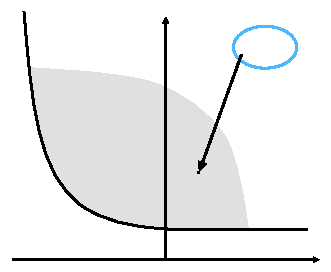
\includegraphics{part_2/chapter_8/figures/generic_G.pdf}};
%		\draw[help lines] (-2,-2) grid (2,2);
		\node[right] at (1.15, 1.5) {\scriptsize $x \in X$};
		\node[right] at (0.9, 0.4) {\footnotesize $(g(x), f(x))$};
		\node[right] at (-2.2, 0.9) {$G$};
		\node[right] at (0,-1.35) {\footnotesize $(\overline{y}, \overline{z}) = (g(\overline{x}), f(\overline{x}))$};
		\node[right] at (2,-1.9) {\footnotesize $y=g(x)$}; 
		\node[right] at (-0.2,2.15) {\footnotesize $z = f(x)$};
	\end{tikzpicture}
	\caption{Illustration of the mapping $G$, in which one can see that solving $P$ amounts to finding the lowermost point on the vertical axis (the ordinate) that is still contained within $G$.} \label{fig:generic_G}	
\end{figure}
%

Now, assume that $u \geq 0$ is given. The Lagrangian function is given by 
$$
\theta(u) = \min_x \braces{f(x) + ug(x) : x \in X}, 
$$ which can be represented by a hyperplane of the form $z = \alpha - uy$. Therefore, optimising the Lagrangian dual problem $(D) : \sup_u \braces{\theta(u)}$ consists of finding the slope $-u$ that would achieve the maximum intercept on the ordinate $z$ while being a supporting hyperplane for $G$. Figure \ref{fig:convex_G} illustrates this effect. Notice that, in this case, the optimal values of the primal and dual problems coincide.
%
\begin{figure}
		\begin{tikzpicture}
			\node at (0,0) {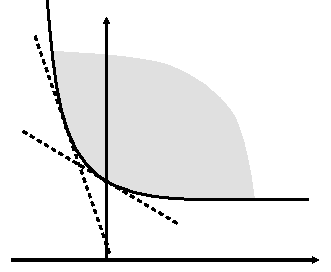
\includegraphics{part_2/chapter_8/figures/convex_G.pdf}};
			\node[right] at (-1.2,2.15) {\footnotesize $z = f(x)$};
			\node[right] at (2,-1.9) {\footnotesize $y=g(x)$}; 
			\node at (0, 0.5) {$G$};
			\node[right] at (0.2,-1.4) {\footnotesize $z + \overline{u}y = \alpha$};
			\node[left] at (-1.3,-1) {\footnotesize $z + uy = \alpha$};
			\node[right] at (-1,-1.9) {\footnotesize $\theta(u)$};
			\node[right] at (-1,-0.6) {\footnotesize $(\overline{y}, \overline{z}) = (g(\overline{x}), f(\overline{x})=\theta(\overline{u})$};		
	%		\draw[help lines] (-2,-2) grid (2,2);		
		\end{tikzpicture}
		\caption{Solving the Lagrangian dual problem is the same as finding the coefficient $u$ such that $z = \alpha - uy$ is a supporting hyperplane of $G$ with the uppermost intercept $\alpha$. Notice that, for $\overline{u}$, the hyperplane supports $G$ at the same point that solves $P$.}\label{fig:convex_G}
	\end{figure}
%
The \emph{perturbation function} $v(y) = \mini\braces{f(x) : g(x) \leq y, x \in X}$ is an analytical tool that plays an important role in understanding when strong duality holds, which, in essence, is the underlying reason why the optimal values of the primal and dual problems coincide. 

Specifically, notice that $v(y)$ is the greatest monotone nonincreasing lower envelope of $G$. Moreover, the reason why $f(\overline{x}) = \theta(\overline{u})$ is related to the convexity of $v(y)$, which implies that 
$$
	v(y) \geq v(0) - \overline{u}y \text{ for all } y \in \reals.
$$

Notice that this is a consequence of Theorem 12 from Lecture 2 (that states that convex sets have supporting hyperplanes for all points on their boundary) and Theorem 5 in Lecture 3 (that convex functions have convex epigraphs)

A \emph{duality gap} exists when the perturbation function $v(y)$ does not have supporting hyperplanes within all its domain, which is otherwise the case when $v(y)$ is convex. Figure \ref{fig:nonconvex_G} illustrates a case in which $v(y)$ is not convex and therefore $\theta(\overline{u}) < f(\overline{x})$.

\begin{figure}[h]
			\begin{tikzpicture}
				\node at (0,0) {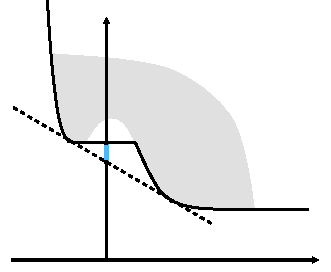
\includegraphics{part_2/chapter_8/figures/nonconvex_G.pdf}};
				\node[right] at (-1.2,2.15) {\footnotesize $z = f(x)$};
				\node[right] at (2,-1.9) {\footnotesize $y=g(x)$}; 
				\node at (0, 0.8) {$G$};
				\node[left] at (0.75,-1.5) {\footnotesize $z + \overline{u}y = \alpha$};
				\node[left] at (-0.9,-0.65) {\footnotesize $\theta(\overline{u})$};
				\node[right] at (-1.1,0.1) {\footnotesize $(\overline{y}, \overline{z}) = (g(\overline{x}), f(\overline{x})$};		
%				\draw[help lines] (-2,-2) grid (2,2);		
			\end{tikzpicture} \label{fig:nonconvex_G}
			\caption{An example in which the perturbation function $v(y)$ is not convex. Notice the consequent mismatch between the intercept of the supporting hyperplane and the lowermost point on the ordinate still contained in $G$.} \label{fig:nonconvex_G}
	\end{figure}


Let us illustrate the above with two numerical examples. First, consider the following problem
%
\begin{align*}
	(P):~ \mini \ & x_1^2 + x_2^2 \\
	& x_1 + x_2 \geq 4 \\
	& x_1, x_2 \geq 0.
\end{align*}
%
The Lagrangian dual function is given by 
%
\begin{align*} 
	(D):~\theta(u) & = \inf \braces{x_1^2 + x_2^2 + u(-x_1 -x_2 + 4) : x_1, x_2 \geq 0} \\
	& = \inf \braces{x_1^2 - ux_1 : x_1 \geq 0} + \inf \braces{x_2^2 - ux_2 : x_2 \geq 0} + 4u \\
	& = \begin{cases}
	     -1/2u^2 + 4u, \text{ if } u \geq 0 \\
	     -4u, ~\, 1 + 4u^2 \text{ if } u < 0. 
	 \end{cases}
\end{align*}

\begin{figure}
	\centering
	\begin{subfigure}{0.45\textwidth}
		\centering
		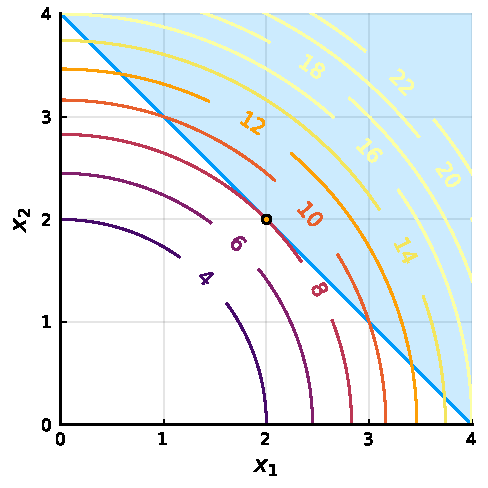
\includegraphics[width=\textwidth]{part_2/chapter_8/figures/ex1_1.pdf}
		\caption{$P$}\label{fig:ex1_P}
	\end{subfigure}
	\begin{subfigure}{0.45\textwidth}
		\centering
		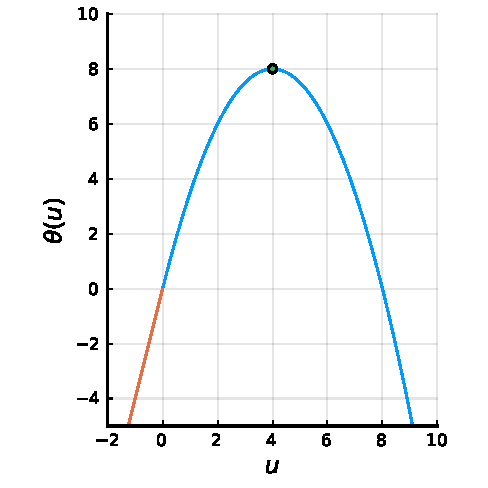
\includegraphics[width=\textwidth]{part_2/chapter_8/figures/ex1_2.pdf}
		\caption{$D$}\label{fig:ex1_D}
	\end{subfigure}
	\caption{The primal problem $P$ as a constrained optimisation problem, and the dual problem $D$, as an unconstrained optimisation problem. Notice how the Lagrangian dual function is discontinuous, due to the implicit minimisation in $x$ of $\theta(u) = \inf_{x \in X} \phi(x,u)$.}	
\end{figure}

Figures \ref{fig:ex1_P} and \ref{fig:ex1_D} provide a graphical representation of the primal problem $P$ and dual problem $D$. As can be seen, both problems have as optimal value $f(\overline{x}_1,\overline{x}_2) = \theta(\overline{u}) = 8$, with the optimal solution $\overline{x} = (2,2)$ for $P$ and $\overline{u} = 4$ for $D$.

To draw the $(g,f)$ map of $X$, we proceed as follows. First, notice that 
$$
v(y) = \mini \braces{x_1^2 + x_2^2 : -x_1 -x_2 + 4 \geq y}
$$
which shows that $(x_1, x_2) = (0,0)$ if $y > 4$. For $y \le 4$, $v(y)$ can be equivalently rewritten as
$$
v(y) = \mini \braces{x_1^2 + x_2^2 : -x_1 -x_2 + 4 = y}.
$$
Let $h(x) = -x_1 - x_2 + 4$ and $f(x) = x_1^2 + x_2^2$. Now, the optimality conditions for $\overline{x}$ to be an optimum for $v$ are such that
$$
\nabla f(\overline{x}) + u \nabla h(\overline{x}) = 0 \Rightarrow \begin{cases} 2x_1 - u = 0 \\ 2x_2 - u =0\end{cases} \Rightarrow	\overline{x}_1  = \overline{x}_2 = u/2.
$$

From the definition of $h(x)$, we see that $u = 4-y$, and thus $\overline{x} = (\frac{4-y}{2}, \frac{4-y}{2})$, which, substituting in $f(x)$ gives $v(y) = (4-y)^2/2$. Note that $v(y) \geq v(0) - \overline{u}y$ holds for all $y \in \reals$, that is, $v(y)$ is convex. Also, notice that the supporting hyperplane is exactly $z = 8 -4y$. 

\begin{figure}
	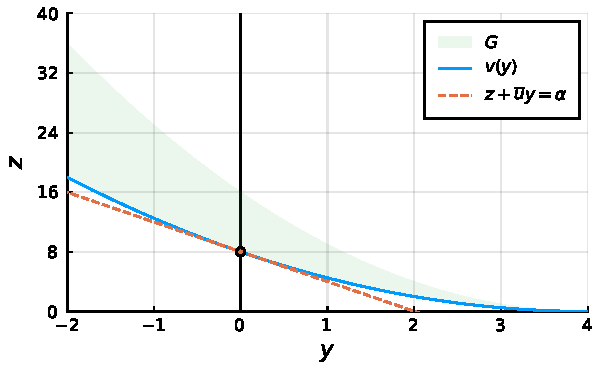
\includegraphics[width = 0.65\textwidth]{part_2/chapter_8/figures/ex1_3.pdf}
	\caption{The $G$ mapping for the first example.}	
\end{figure}

Now, let us consider a second example, in which the feasible set is not convex and, therefore, the mapping $G$ will not be convex either. For that, consider the problem
%
\begin{align*}
	(P):~ \mini \ & -2x_1 + x_2 \\
	\st & x_1 + x_2 = 3 \\
	& x_1, x_2 \in X.
\end{align*}
%
where $X = \braces{(0,0), (0,4), (4,4), (4,0), (1,2), (2,1)}$. The optimal point $\overline{x} = (2,1)$. The Lagrangian dual function is given by
\begin{align*} 
	\theta(v) & = \min \braces{ (-2x_1 + x_2) + v(x_1 + x_2 - 3) : (x_1, x_2) \in X} \\
	& = \begin{cases}
	     -4 + 5v, \text{ if } v \leq -1 \\
	     -8 + v, 5 \text{ if }  -1 \leq v \leq 2 \\
	     -3v, + p_1 \text{ if } v \geq 2. 
	 \end{cases}
\end{align*} 

Figure \ref{fig:ex2_P} provides a graphical representation of the problem. Notice that to obtain the Lagrangian dual function one must simply take the lowermost segments of the hyperplanes obtained when considering each $x \in X$, which leads to a piecewise concave function, as represented in Figure \ref{fig:ex2_D}. 

\begin{figure}[h]
	\centering
	\begin{subfigure}{0.45\textwidth}
		\centering
		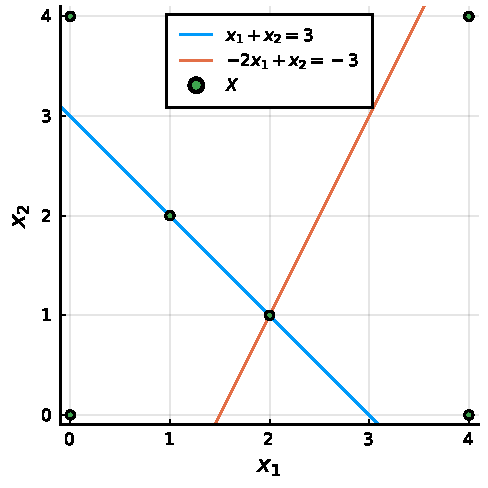
\includegraphics[scale=0.8]{part_2/chapter_8/figures/ex2_1.pdf}
		\caption{$P$} \label{fig:ex2_P}	
	\end{subfigure}
	\begin{subfigure}{0.45\textwidth}
		\centering
		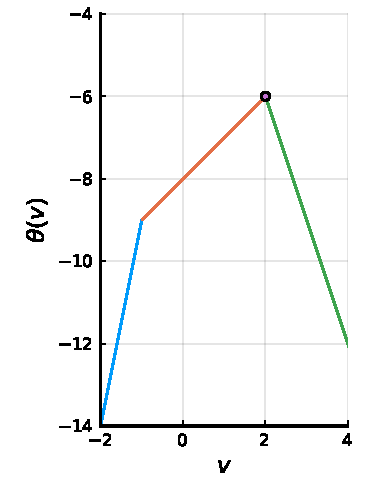
\includegraphics[scale=0.8]{part_2/chapter_8/figures/ex2_2.pdf}
		\caption{$(D): \maxi \theta(v)$} \label{fig:ex2_D}	
	\end{subfigure}
	\caption{The primal problem $P$ as a constrained optimisation problem and the dual problem $D$. Notice how the Lagrangian dual function is concave and piecewise linear, despite the nonconvex nature of $P$.}
\end{figure}

Similarly to the previous example, we can plot the $G$ mapping, which in this case consists of the points $x \in X$ mapped as $(h(x), f(x))$, with $h(x) = x_1 + x_2 - 3$ and $f(x) = -2x_1 + x_2$. Notice that $v(y)$ in this case is discontinuous, represented by the three lowermost points. Clearly, $v(y)$ does not have a supporting hyperplane at the minimum of $P$, which illustrates the existence of a duality gap, as stated by the fact that $-3 = f(\overline{x}) > \theta(\overline{v}) = -6$. 


\begin{figure}
	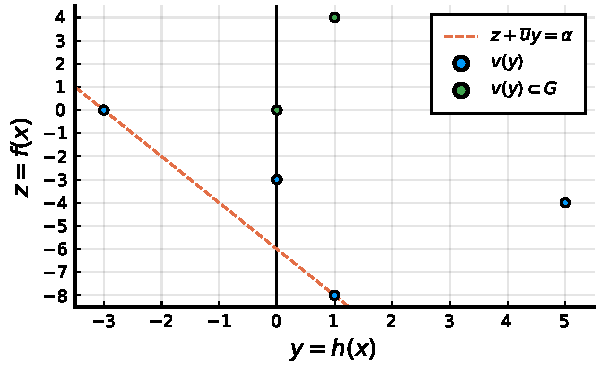
\includegraphics[width=0.65\textwidth]{part_2/chapter_8/figures/ex2_3.pdf}
	\caption{The $G$ mapping for the second example. The blue dots represent the perturbtion function $v(y)$, which is not convex and thus cannot be supported everywhere. Notice the duality gap represented by the difference between the intercept of $z = -6 -2y$ and the optimal value of $P$ at (0,-3).}
\end{figure}
	


\subsubsection{Strong duality}

From the previous graphical interpretation and related examples, it becomes clear that there is a strong tie between strong duality and the convexity of $P$. This is formally described in Theorem \ref{thm:strong_duality}.

\begin{theorem} \label{thm:strong_duality}
	Let $X \subseteq \reals^n$ be a nonempty convex set. Moreover, let $f: \reals^n \rightarrow \reals$ and $g: \reals^n \rightarrow \reals^m$ be convex functions, and let $h: \reals^n \rightarrow \reals^l$ be an affine function: $h(x) = Ax - b$. Suppose that Slater's constraint qualification holds true. Then 
	$$ \inf_{x} \braces{f(x) : g(x) \leq 0, h(x) = 0, x \in X} = \sup_{u,v}\braces{\theta(u,v) : u \geq 0},
	$$ 
	where $\theta(u,v) = \inf_{x \in X} \braces{f(x) + u^\top g(x) + v^\top h(x)}$ is the Lagrangian function. Furthermore, if $\inf_x \braces{f(x) : g(x) \leq 0, h(x) = 0, x \in X}$ is finite and achieved at $\overline{x}$, then \lb $ \sup_{u,v}\braces{\theta(u,v) : u \geq 0}$ is achieved at $(\overline{u},\overline{v})$ with $\overline{u} \geq 0$ and $\overline{u}^\top g(\overline{x}) = 0$.
\end{theorem}

The proof for the strong duality theorem follows the following outline:
%
\begin{enumerate}
	\item Let $\gamma = \inf_x \braces{f(x) : g(x) \leq 0, h(x) = 0, x \in X}$. Suppose that $ -\infty < \gamma < \infty$, hence finite (for unbounded problems, $f(x) = -\infty$ implies $\theta(u,v) = -\infty$ since $\theta(u,v) \leq f(x)$ from Theorem \ref{thm:weak_duality}; the right-hand side holds by assumption of the existence of a feasible point from Slater's constraint qualification).
	\item Formulate the inconsistent system: 
	$$f(x) - \gamma < 0, \quad g(x) \leq 0, \quad h(x) = 0, \quad x \in X.$$
	\item Use the separation theorem (or a variant form of Farkas theorem) to show that $(\overline{u}_0, \overline{u}, \overline{v})$ with $\overline{u}_0 > 0$ and $\overline{u} \geq 0$ exists such that, after scaling using $\overline{u}_0$ one obtains 
	$\theta(\overline{u},\overline{v}) := f(x) + \overline{u}^\top g(x) + \overline{v}^\top h(x) \geq \gamma, \ x \in X$, which requires the assumption of Slater's constraint qualification. 
	\item From weak duality (Theorem~\ref{thm:weak_duality}), we have that $\theta(\overline{u},\overline{v}) \leq \gamma$, which combined with the above, yields $\theta(\overline{u},\overline{v}) = \gamma$.
	\item Finally, an optimal $\overline{x}$ solving the primal problem implies that $g(\overline{x}) \leq 0$, $h(\overline{x}) =0$, $\overline{x} \in X$, and $f(x) = \gamma$. From 3, we have $\overline{u}^\top g(\overline{x}) \geq 0$. As $g(\overline{x}) \leq 0$ and $\overline{u}\geq 0$, $\overline{u}^\top g(\overline{x}) \geq 0=0$. 
\end{enumerate}

The proof uses a variant of the Farkas theorem that states the existence of a solution for the system $u_0(f(x) - \gamma) + u^\top g(x) \geq 0, x \in X$ with $(u_0, u, v) \neq 0$, what can be shown to be the case if Slater's constraint qualification holds. This, combined with weak duality stated in Theorem \ref{thm:weak_duality} yields strong duality.  


\subsection{Employing Lagrangian duality for solving optimisation problems}

Weak duality can be used to derive a stopping criterion for solution methods that can generate both primal and dual feasible solutions, also known as primal-dual pairs. Such methods are typically referred to as primal-dual methods, being the primal-dual interior point method (which we will discuss in details in an upcoming lecture) perhaps the most widely known.
	
For feasible $x$ and $(u,v)$, one can bound how suboptimal $f(x)$ is, by noticing that
	$$
		f(x) - f(\overline{x}) \le f(x) - \theta(u,v),
	$$
	which is a consequence of $f(\overline{x}) \ge \theta(u,v)$ (i.e., weak duality). We say that $x$ is $\epsilon$-optimal, with $\epsilon = f(x) - \theta(u,v)$. 

In essence, $(u,v)$ is a certificate of (sub-)optimality of $x$, as $(u,v)$ proves that $x$ is $\epsilon$-optimal. Moreover, in case strong duality holds, under the conditions of Theorem 6, one can expect $\epsilon$ converge to zero.

To see how this the case, observe the following. First, as can be seen in Theorem \ref{thm:strong_duality}, a consequence of strong duality is that complementarity conditions $\overline{u}^\top g(\overline{x}) \geq 0=0$ hold for an optimal primal-dual pair $(\overline{x} , (\overline{u}, \overline{v}))$. Secondly, notice that, by definition, $\overline{x}$ and $(\overline{u}, \overline{v})$ are primal and dual feasible, respectively. 

The last component missing is to notice that, if $\overline{x}$ is a minimiser for $\phi(x,\overline{u},\overline{v}) = f(x)  + \overline{u}^\top g(x) + \overline{v}^\top h(x) $, then we must have
		$$
		\nabla f(\overline{x}) + \sum_{i=1}^m u_i \nabla g_i(\overline{x}) + \sum_{i=1}^{l} v_i \nabla h_i(\overline{x})= 0.
		$$  

Combining the above, one can see that we have listed all of the KKT optimality conditions, which under the assumptions of Theorem \ref{thm:strong_duality} are known to be necessary and sufficient for global optimality. That is, in this case, any primal dual pair for which the objective function values match will automatically be a point satisfying the KKT conditions and therefore globally optimal. This provides an alternative avenue to search for optimal solutions, relying on Lagrangian dual problems. 

\subsection{Saddle point optimality and KKT conditions*}

An alternative perspective for establishing necessary and sufficient conditions for strong duality to hold involves identifying the existence of saddle points for the Lagrangian dual problem.

Let us first define saddle points in the context of Lagrangian duality. Let 
$$
(P) :~ \mini\braces{f(x) : g(x) \leq 0, h(x) = 0, x \in X}.
$$ 
Let us define the Lagrangian function $\phi(x,u,v) = f(x)  + u^\top g(x) + v^\top h(x) $. A solution $(\overline{x}, \overline{u}, \overline{v})$ is called a \emph{saddle point} if $\overline{x} \in X$, $\overline{u} \geq 0$, and 
$$ 
\phi(\overline{x},u,v)  \leq \phi(\overline{x}, \overline{u}, \overline{v})  \leq \phi(x,\overline{u}, \overline{v}) 
$$
for all $x \in X$ and  $(u,v)$ such that $u \geq 0$. 

Notice that this definition implies that:
\begin{itemize}
\item $\overline{x}$ minimises $\phi(x,u,v)$ when $(u,v)$ is fixed at $(\overline{u}, \overline{v})$; 
\item $(\overline{u}, \overline{v})$ maximises $\phi(x,u,v)$ when $x$ is fixed at $\overline{x}$.
\end{itemize}

This insight allows for the development of methods that can alternatively solve the Lagrangian dual problem in the space of primal variables $x$ and dual variables $(u,v)$ in a block-coordinate descent fashion. 

Theorem \ref{thm:saddle_point} establishes the relationship between the existence of saddle points for Lagrangian dual problems and zero duality gaps.

\begin{theorem}[Saddle point optimality and zero duality gap] \label{thm:saddle_point}

A solution $(\overline{x}, \overline{u}, \overline{v})$ with $\overline{x} \in X$ and $\overline{u} \geq 0$ is a saddle point for the Lagrangian function $\phi(x,u,v) = f(x)  + u^\top g(x) + v^\top h(x) $ if and only if:
\begin{enumerate}
\item $\phi(\overline{x}, \overline{u}, \overline{v}) = \mini\braces{\phi(x, \overline{u}, \overline{v}): x \in X}$
\item $g(\overline{x}) \leq 0$, $h(\overline{x}) = 0$, and 
\item $\overline{u}^\top g(\overline{x}) = 0$
\end{enumerate}
Moreover, $(\overline{x}, \overline{u}, \overline{v})$ is a saddle point if and only if $\overline{x}$ and $(\overline{u}, \overline{v})$ are optimal solutions for the primal (P) and dual (D) problems, respectively, with $f(\overline{x}) = \theta(\overline{u}, \overline{v})$. 
\end{theorem}

From Theorem \ref{thm:saddle_point} it becomes clear that there is a strong connection between the existence of saddle points and the KKT conditions for optimality. Figure \ref{KKT_saddle} illustrates the existence of a saddle point and the related zero optimality gap.

\begin{figure}[H]
	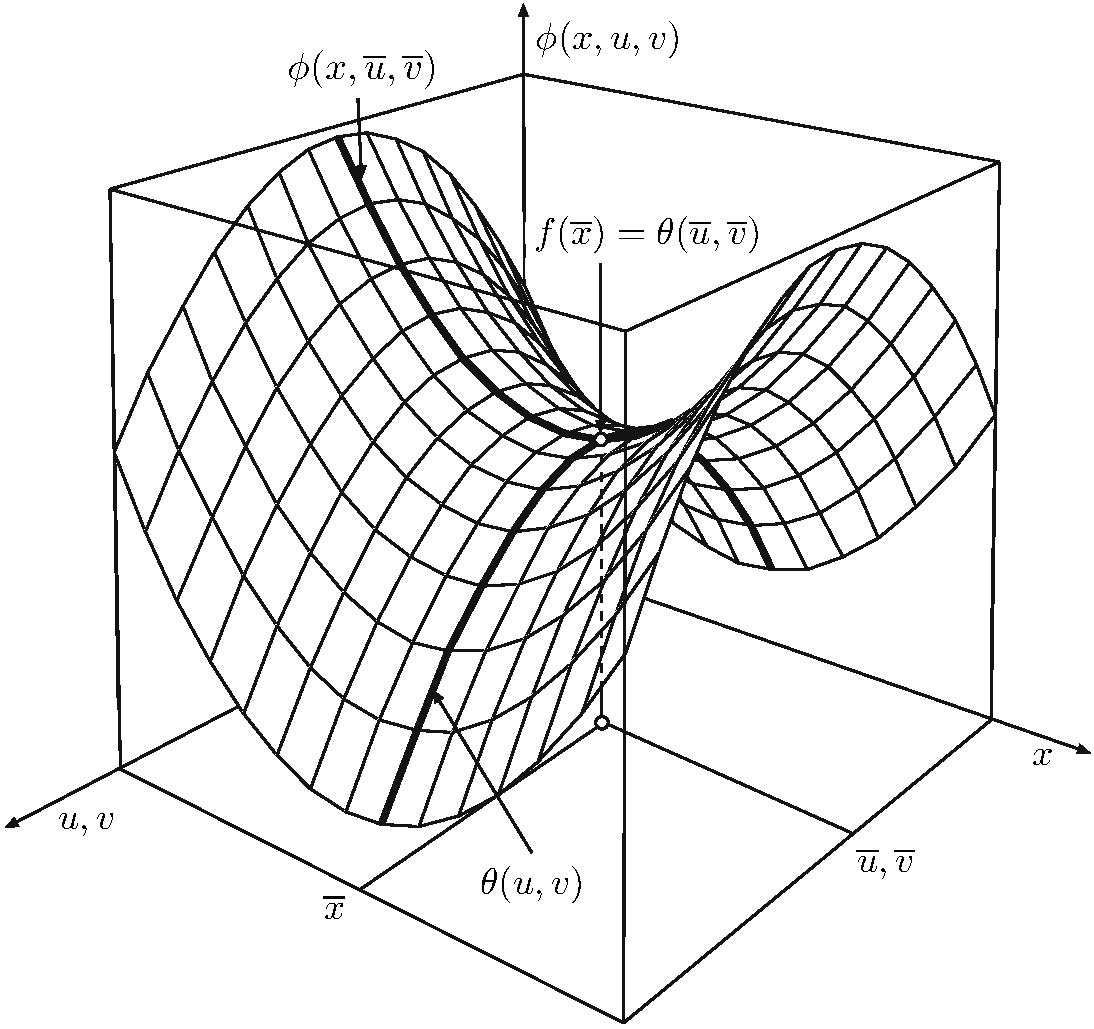
\includegraphics[width=0.7\textwidth]{part_2/chapter_8/figures/KKT_saddle.pdf}
	\caption{Illustration of a saddle point for the Lagrangian dual problem}\label{KKT_saddle}
\end{figure}



%% Fix this

%\begin{longproof}
%{\bf Part 1:} suppose $(\overline{x}, \overline{u}, \overline{v})$ is a saddle point. Then {\color{blue}1} must be true. Moreover\\[-6pt]
%$$ f(\overline{x}) + \overline{u}^\top g(\overline{x}) + \overline{v}^\top h(\overline{x}) \geq f(\overline{x}) + u^\top g(\overline{x}) + v^\top h(\overline{x}) 
%$$ for all $(u,v)$ with $u \geq 0$. This implies that $g(\overline{x}) \leq 0$ and $h(\overline{x}) = 0$; otherwise, this can be violated with large enough $(u,v)$. Now, by setting $u=0$, we notice that $\overline{u}^\top g(\overline{x}) \geq 0$, and thus $\overline{u}^\top g(\overline{x}) = 0$.\\[6pt] 
%
%\pause
%Conversely, assume that {\color{blue}1}, {\color{blue}2}, and {\color{blue}3} hold true for a given $(\overline{x}, \overline{u}, \overline{v})$ with $u \geq 0$. Then $(\overline{x}, \overline{u}, \overline{v}) \leq (x, \overline{u}, \overline{v})$ for all $x \in X$ by {\color{blue}1}. Also, 
%\begin{align*}
%\phi(\overline{x}, \overline{u}, \overline{v}) &= f(\overline{x}) + \overline{u}^\top g(\overline{x}) + \overline{v}^\top h(\overline{x}) \\ 
%&= f(\overline{x}) \geq f(\overline{x}) + u^\top g(\overline{x}) + v^\top h(\overline{x}) = \phi(\overline{x}, u, v)
%\end{align*}
%for all $(u,v)$ with $u \geq 0$, and hence $(\overline{x}, \overline{u}, \overline{v})$ is a saddle point.
%\end{longproof}
%
%\end{frame}
%
%
%\begin{frame}{Saddle points in Lagrangian dual functions}
%
%\begin{proof}[\proofname\ (cont.)]
%{\bf Part 2:} Once again, assume that $(\overline{x}, \overline{u}, \overline{v})$ is a saddle point. By {\color{blue}2}, $\overline{x}$ is feasible to $P$ and, by assumption, $(u,v)$ with $\overline{u} \geq 0$ is feasible to $D$. Properties {\color{blue}1}, {\color{blue}2}, and {\color{blue}3} imply that 
%\vspace{-6pt}
%$$ \theta(\overline{u},\overline{v}) = \phi(\overline{x}, \overline{u}, \overline{v}) = f(\overline{x}) + \overline{u}^\top g(\overline{x}) + \overline{v}^\top h(\overline{x}) = f(\overline{x}). \vspace{-12pt}
%$$\\[6pt]
%From {\color{blue}Corollary~\ref{cor:strong_duals}}, $\overline{x}$ and $(\overline{u},\overline{v})$ solve $P$ and $D$ with no duality gap.
%
%\pause
%Now, assume that $\overline{x}$ and $(\overline{u}, \overline{v})$ solve $P$ and $D$, with $\theta(\overline{u},\overline{v}) = f(\overline{x})$. Thus,  $\overline{x} \in X$, $g(\overline{x}) \leq 0$, $h(\overline{x}) = 0$, and $\overline{u} \geq 0$. Also,  
%\vspace{-6pt}
%\begin{align*} 
%\theta(\overline{u},\overline{v}) &= \inf\braces{f(x) + \overline{u}^\top g(x) + \overline{v}^\top h(x) : x \in X} \\
%&\leq f(\overline{x}) + \overline{u}^\top g(\overline{x}) + \overline{v}^\top h(\overline{x}) \leq f(\overline{x}).
%\end{align*}\\[-6pt]
%%
%Equality holds by assumption, thus implying that $\overline{u}^\top g(\overline{x}) = 0$ and $\phi(\overline{x}, \overline{u}, \overline{v})= f(\overline{x}) = \theta(\overline{u}, \overline{v}) = \inf\braces{\phi(x, \overline{u}, \overline{v}) : x \in X}$. Therefore, {\color{blue}1}, {\color{blue}2}, and {\color{blue}3} hold.
%\end{proof}


\section{Properties of Lagrangian functions}


Lagrangian duals are a useful framework for devising solution methods for constrained optimisation problems if solving the dual problem can be done efficiently or exposes some exploitable structure.

One important property that Lagrangian dual functions present is that they are \emph{concave piecewise linear} in the dual multipliers. Moreover, they are continuous and thus have subgradients everywhere. Notice however that they are typically not differentiable, requiring the employment of a \emph{nonsmooth optimisation} method to be appropriately solved. Theorem \ref{thm:Lagrangian_dual_concave} establishes the concavity of the Lagrangian dual function.

\begin{theorem}[Concavity of Lagrangian dual functions]\label{thm:Lagrangian_dual_concave}
Let $X \subseteq \reals^n$ be a nonempty compact set, and let $f: \reals^n \rightarrow \reals$ and $\beta : \reals^{n} \rightarrow \reals^{m+l}$, with $w^\top\beta(x) = \binom{u}{v}^\top \binom{g(x)}{h(x)}$ be continuous. Then $\theta(w) = \inf_x\braces{f(x) + w^\top\beta(x) : x \in X}$ is concave in $\reals^{m+l}$
\end{theorem}

\begin{proof}
Since $f$ and $\beta$ are continuous and $X$ is compact, $\theta$ is finite on $R^{m+l}$. Let $w_1$, $w_2 \in \reals^{m+l}$, and let $\lambda \in (0,1)$. We have
\begin{align*}
&\theta[\lambda w_1 + (1 - \lambda)w_2] = \inf_x\braces{f(x) + [\lambda w_1 + (1 - \lambda)w_2]^\top \beta(x) : x \in X}\\
& = \inf_x\braces{\lambda[f(x) + w_1^\top\beta(X)] + (1-\lambda)[f(x) + w_2^\top \beta(x)] : x \in X} \\
& \geq \lambda \inf_x\braces{f(x) + w_1^\top \beta(x) : x \in X} + (1 - \lambda)\inf_x\braces{f(x) + w_2^\top \beta(x) : x \in X} \\
&= \lambda \theta(w_1) + (1 - \lambda) \theta(w_2). \qedhere
\end{align*}
\end{proof}

The proof uses the fact that the Lagrangian function $\theta(w)$ is the infimum of affine functions in $w$, and therefore concave. An alternative approach to show the concavity of the Lagrangian function is to show that it has subgradients everywhere. This is established in Theorem \ref{thm:Lagrangian_dual_subgradient}. 

\begin{theorem} \label{thm:Lagrangian_dual_subgradient}
Let $X \subset \reals^n$ be a nonempty compact set, and let $f: \reals^n \mapsto \reals$ and $\beta : \reals^{n} \mapsto \reals^{m+l}$, with $w^\top\beta(x) = \binom{u}{v}^\top \binom{g(x)}{h(x)}$ be continuous. If $\overline{x} \in X(\overline{w}) = \braces{x \in X : x = \arg \min \braces{f(x) + w^\top\beta(x)}}$, then $\beta(\overline{x})$ is a subgradient of $\theta(\overline{w})$.
\end{theorem}
%
\begin{proof}
Since $f$ and $\beta$ are continuous and $X$ is compact, $X(\overline{w}) \neq \emptyset$ for any $w \in \reals^{m+l}$. Now, let $\overline{w} \in \reals^{m+l}$ and $\overline{x} \in X(\overline{w})$. Then
\begin{align*}
\theta(w)& = \inf\braces{f(x) + w^\top\beta(x) : x \in X} \\ & \leq f(\overline{x}) + w^\top\beta(\overline{x}) \\ 
& = f(\overline{x}) + (w - \overline{w})^\top\beta(\overline{x}) + \overline{w}^\top \beta(\overline{x}) \\
& = \theta(\overline{w}) + (w - \overline{w})^\top \beta(\overline{x}). \qedhere
\end{align*}
\end{proof}

Theorem \ref{thm:Lagrangian_dual_subgradient} can be used to derive a simple optimisation method for Lagrangian functions using subgradient information that is easily available from the term $\beta(w)$.


\subsection{The subgradient method}


One challenging aspect concerning the solution of Lagrangian dual functions is that very often they are not differentiable. This requires an adaptation of the gradient method to consider subgradient information instead.

The challenge with using subgradients (instead of gradients) is that subgradients are not guaranteed to be descent directions (as opposed to gradients being the steepest descent direction under adequate norm). Nevertheless, for suitable step size choices, convergence can be observed. Figure \ref{fig:subgradients} illustrates the fact that subgradients are not necessarily descent directions.

\begin{figure}[h]
	\begin{tikzpicture}
		\node at (0,0) {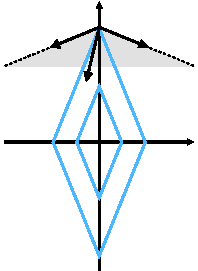
\includegraphics{part_2/chapter_8/figures/nonsmooth.pdf}};
		\node at (1.5, 0.1) {\footnotesize$u_1$};
		\node[right] at (0, 2.2) {\footnotesize$u_2$};
		\node[right] at (0.5, 0.95) {\footnotesize$\partial\theta(w_k)$};
		\node at (-0.5, 0.7) {\footnotesize$\beta(x_k)$};
		\node[above right] at (-0.05, -0.1) {\footnotesize$\overline{w}$};
%		\draw[help lines] (-1,-2) grid (1,2);	
	\end{tikzpicture}
	\caption{One possible subgradient $\beta(x_k)$ that is a descent direction for suitable step size. Notice that within the subdifferential $\partial \theta(w_k)$ other subgradients that are not descent direction are available.} \label{fig:subgradients}	
\end{figure}




Algorithm \ref{Alg1} summarises the subgradient method. Notice that the stopping criterion emulates the optimality condition $0 \in \partial\theta(w_k)$, but in practice, one also enforces more heuristically driven criteria such as maximum number of iterations or a given number of iterations without observable improvement on the value of $\theta(w)$. 

\begin{algorithm}[H]
\caption{Subgradient method} \label{Alg1}
\begin{algorithmic}[1] 
\State {\bf initialise.} tolerance $\epsilon > 0$, initial point $w_0$, iteration count $k = 0$. 
\While {$||\beta(x_k) ||_2 > \epsilon$} 
        \State $x_k \gets \arg \min_x \braces{\theta(w_k) = \inf_x \braces{f(x) + w_k^\top\beta(x)}}$ 
        \State $LB_k = \max \braces{LB_k, \theta(w_k)}$
        \State update $\lambda_k$ \label{alg1:step_update}
        \State $w_{k+1} = w_k + \lambda_k  \beta(x_k)$.
    \State $k \leftarrow k+1$.    
    %\State $k = k+1$
\EndWhile
\State {\bf return} $LB_k = \theta(w_k)$.
\end{algorithmic}
\end{algorithm}

One critical aspect associated with the subgradient method is the step size update described in Step \ref{alg1:step_update} of Algorithm \ref{Alg1}. Theoretical convergence is guaranteed if Step \ref{alg1:step_update} generates a sequence $\braces{\lambda_k}$ such that
$\sum_{k=0}^{\infty}\lambda_k \rightarrow \infty \text{ and } \lim_{k \rightarrow \infty}\lambda_k = 0$. However, discrepant performance can be observed for distinct parametrisation of the method.

The classical step update rule employed for the subgradient method is known as the Polyak rule, which is given by
$$
\lambda_{k+1} = \frac{\alpha_k(LB_k - \theta(w_k))}{||\beta(x_k)||^2}
$$ 
with $\alpha_k \in (0,2)$ and $LB_k$ being the best-available lower-estimate of $\theta(\overline{w})$. This rule is inspired by the following result.

\begin{proposition}[Improving step size]
If $w_k$ is not optimal, then, for all optimal dual solutions $\overline{w}$, we have
\vspace{-6pt}
%
$$|| w_{k+1} - \overline{w}|| < || w_{k} - \overline{w}||$$
%
\vspace{-6pt}
for all step sizes $\lambda_k$ such that 
%
$$0 < \lambda_k < \frac{2(\theta(\overline{w}) - \theta(w_k))}{||\beta(x_k)||^2}.$$
\end{proposition}

\begin{proof}
We have that $|| w_{k+1} - \overline{w} ||^2 = || w_k + \lambda_k\beta(x_k) - \overline{w} ||^2 = $ 
%
$$|| w_{k} - \overline{w}||^2 - 2\lambda_k(\overline{w} - w_k)^\top \beta(x_k) + (\lambda_k)^2||\beta(x_k)||^2.$$
%
By the subgradient inequality: $\theta(\overline{w}) - \theta(w_k) \leq (\overline{w} - w_k)^\top \beta_k$. Thus
%
$$|| w_{k+1} - \overline{w} ||^2 \leq || w_{k} - \overline{w}||^2 - 2\lambda_k(\theta(\overline{w}) - \theta(w_k))^\top \beta(x_k) + (\lambda_k)^2||\beta(x_k)||^2.$$
%
Parametrising the last two terms by $\gamma_k = \frac{\lambda_k ||\beta(x_k)||^2}{\theta(\overline{w}) - \theta(w_k)}$ leads to
%
$$|| w_{k+1} - \overline{w} ||^2 \leq || w_{k} - \overline{w} ||^2 - \frac{\gamma_k(2-\gamma_k)(\theta(\overline{w}) - \theta(w_k))^2}{||\beta(x_k)||^2}.$$
%
Notice that if $0 < \lambda_k < \frac{2(\theta(\overline{w}) - \theta(w_k))}{||\beta(x_k)||^2}$ then $0 < \gamma_k < 2$ and, thus, $|| w_{k+1} - \overline{w}|| < || w_{k} - \overline{w}||$.
\end{proof}

In practice, since $\theta(\overline{w})$ is not known, it must be replaced by a proxy $LB_k$, which is chosen to be a lower bound on $\theta(\overline{w})$ to still satisfy the subgradient inequality. The $\alpha_k$ is then reduced from the nominal value 2 to correct for the estimation error of term $\theta(\overline{w}) - \theta(w_k)$.
